\documentclass[12pt, letterpaper]{article} 

\usepackage{amsmath, amssymb, amsthm, enumerate, graphicx}

\title{MATH 189 HW 5}
\author{Dani Nguyen}
\date{Winter 2025}

\begin{document}
\maketitle
\graphicspath{ {./} }

\noindent \textbf{Question 1} \\
Since boosting takes linear combinations of depth-one trees, which are univariate functions, we get the 
sum of univariate functions, which is just an additive model. \\

\noindent \textbf{Question 2} \\
We split each cell by finding the predictor $X_j$ and cutpoint $s$ that minimizes 
\begin{align*}
    \sum_{i:X_{ij}<s}(Y_i - \hat Y_{R_1})^2 + \sum_{i:X_{ij}\ge s}(Y_i - \hat Y_{R_2})^2
\end{align*}

\newpage
\noindent \textbf{Question 3} \\
\begin{enumerate}[a.]
    \item 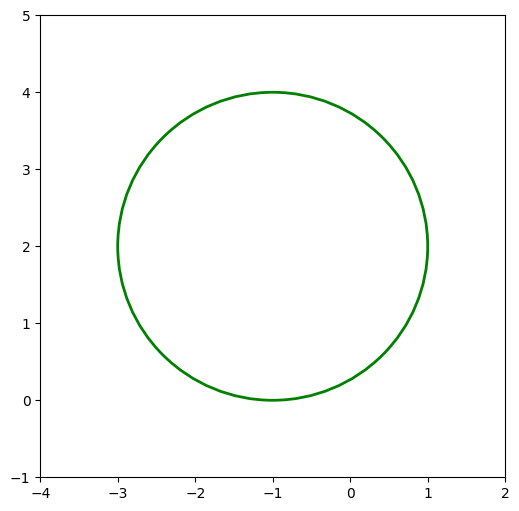
\includegraphics[scale=0.7]{3a.png} 
    \item The set of points for which $(1+X_1)^2 + (2-X_2)^2 > 4$ are the points outside the circle, 
    whereas the set of points for which $(1+X_1)^2 + (2-X_2)^2 \le 4$ are the points on and inside 
    the circle.
    \item \begin{tabular}{c |c |c}
        Points & $(1+X_1)^2 + (2-X_2)^2$ & Class\\
        \hline 
        (0,0) & 5 & Blue \\
        (-1,1)& 1 & Red \\
        (2,2) & 9 & Blue\\
        (3,8) & 52& Blue
    \end{tabular}
    \item If we expand the equation for the decision boundary to $5 + 2X_1 - 4X_2 + X_1^2 + X^2_2 = 4$, 
    we get an equation that is linear in terms of $X_1, X_2, X_1^2, X_2^2$
\end{enumerate}

\newpage
\noindent \textbf{Question 4} \\
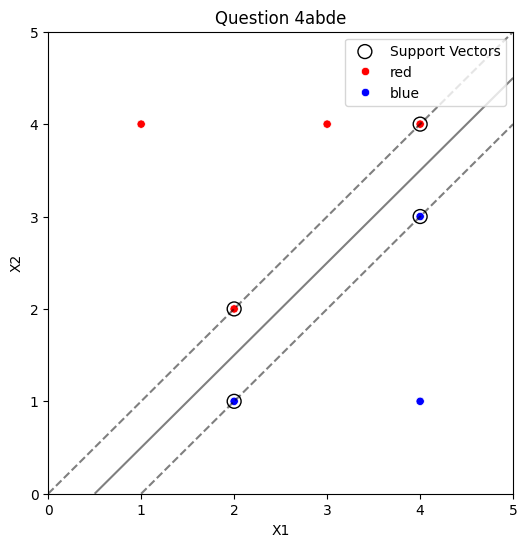
\includegraphics{4abde.png}
\begin{enumerate}
    \item[c.] Classify to Red if $\beta_0 + \beta_1X_1 + \beta_2X_2 > 0$ and Blue otherwise. \\
    In this case, $\beta_0 = -0.5,\ \beta_1 = 1,\ \beta_2 = -1$
    \item[f.] The 7th observation (4,1) if moved slightly will not affect the hyperplane because 
    it is not a support vector, the equation of the hyperplane does not depend on it. 
    \item[g.] The equation for this hyperplane is $0 = 0.8 X_1 - X_2$ \\
    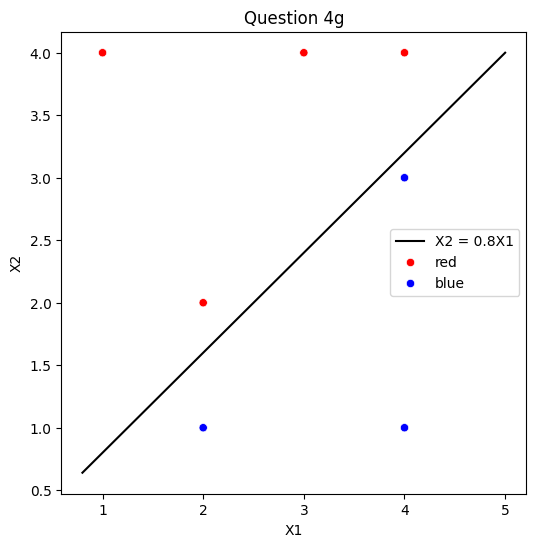
\includegraphics{4g.png} \newpage
    \item[h.] A point that would make the two classes unseparable by a hyperplane would be (2,4) with
    the category Blue. \\
    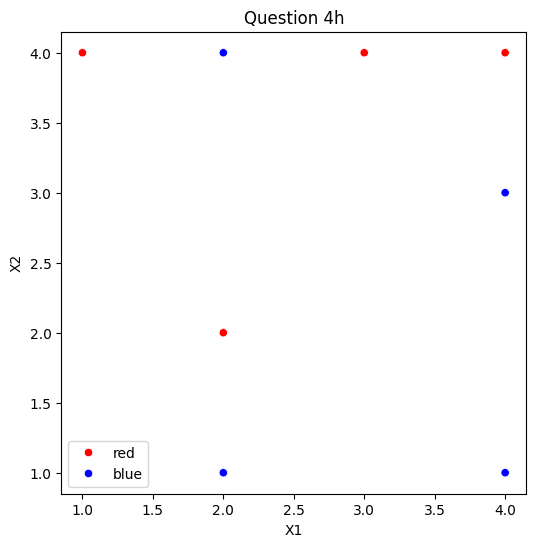
\includegraphics{4h.png}
\end{enumerate}

\newpage
\noindent \textbf{Question 5} \\


\newpage
\noindent \textbf{Question 6} \\
Linear kernel support vector machine \\
Training score: 0.77 \\
Test score: 0.72 \\
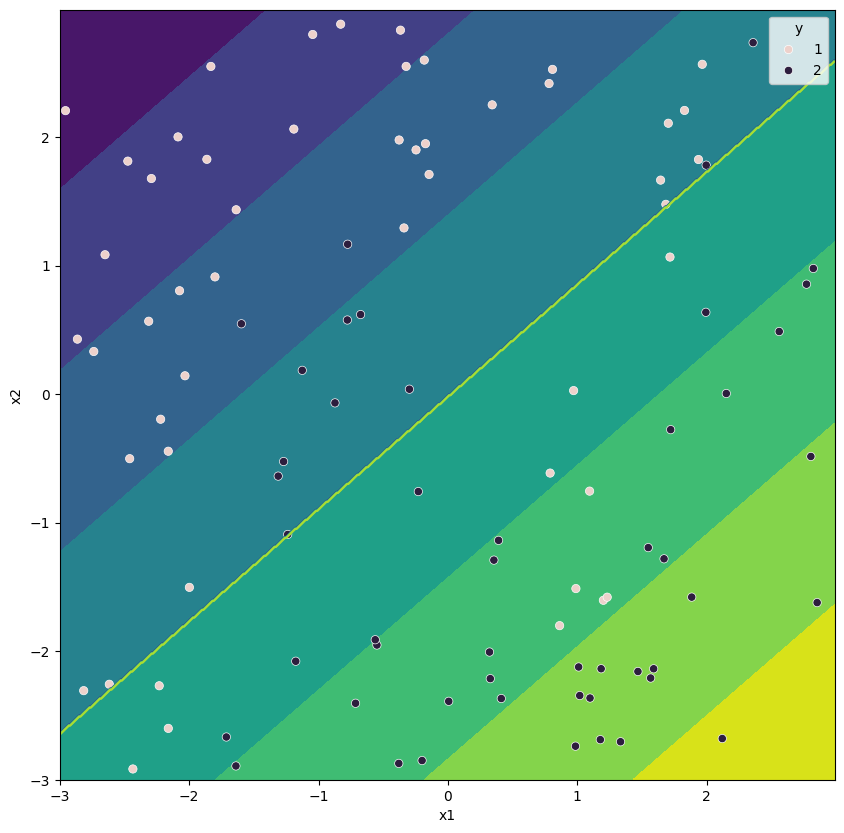
\includegraphics[scale=0.63]{6linear.png} \\
\newpage
\noindent Radial kernel support vector machine \\
Training score: 0.89 \\
Test score: 0.79 \\
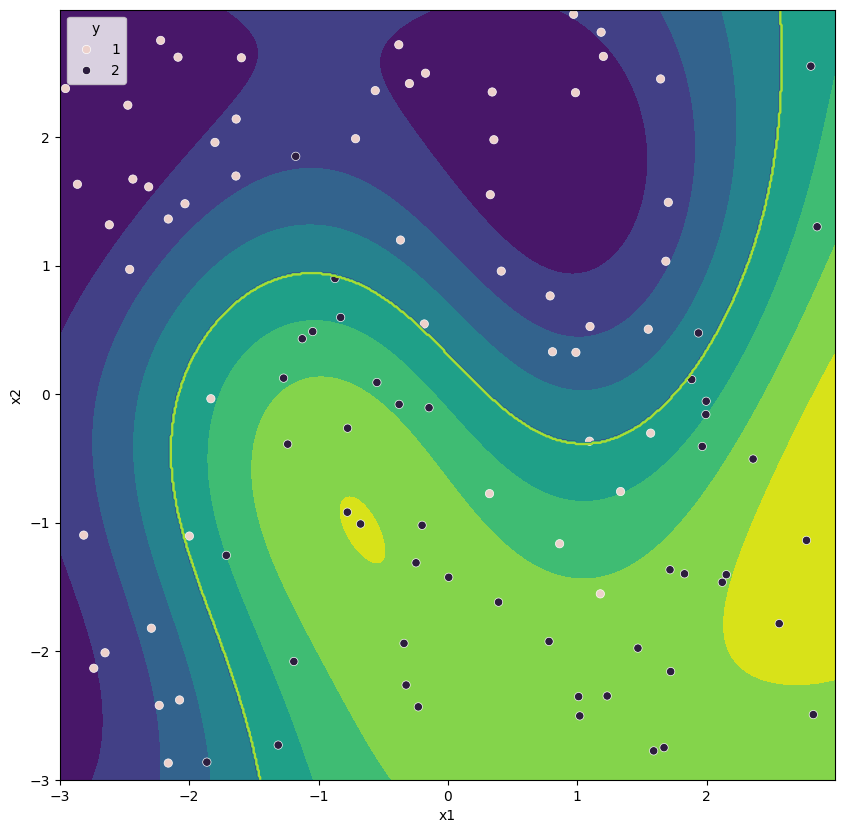
\includegraphics[scale=0.63]{6radial.png} \\
Therefore, radial kernel works better in this case of non-linear separation between the two classes.

\end{document}